%!TEX TS-program = xelatex
%!TEX encoding = UTF-8 Unicode

%%%%%%%%%%%%%%%%%%%%%%%%%%%%%%%%%%%%%%%%%
% Journal Article
% LaTeX Template
% Version 1.4 (15/5/16)
%
% This template has been downloaded from:
% http://www.LaTeXTemplates.com
%
% Original author:
% Frits Wenneker (http://www.howtotex.com) with extensive modifications by
% Vel (vel@LaTeXTemplates.com)
%
% License:
% CC BY-NC-SA 3.0 (http://creativecommons.org/licenses/by-nc-sa/3.0/)
%
%%%%%%%%%%%%%%%%%%%%%%%%%%%%%%%%%%%%%%%%%

%----------------------------------------------------------------------------------------
%	PACKAGES AND OTHER DOCUMENT CONFIGURATIONS
%----------------------------------------------------------------------------------------

\documentclass[
	12pt,
	a4paper,
	%twoside,
	twocolumn
	]{article}

\usepackage{blindtext} % Package to generate dummy text throughout this template

%\usepackage[sc]{mathpazo} % Use the Palatino font
\usepackage[T1]{fontenc} % Use 8-bit encoding that has 256 glyphs
\usepackage[utf8]{inputenc}

\linespread{1.05} % Line spacing - Palatino needs more space between lines
\usepackage{microtype} % Slightly tweak font spacing for aesthetics

\usepackage[english]{babel}

\usepackage[
	%hmarginratio=1:1,
	top=20mm,
	bottom=25mm,
	textwidth=17.2cm,
	columnsep=0.8cm%19pt
	]{geometry} % Document margins

%-------------------------------------------------------------
%----------------------------------------------------- FONTS -
%-------------------------------------------------------------

\linespread{1.04}

\usepackage{paralist}

\usepackage{etoolbox}

\usepackage{fontspec,
			xltxtra,
			xunicode
			}

\defaultfontfeatures{Mapping=tex-text}

\setromanfont[
	Mapping=tex-text
	]{Alegreya}

\setsansfont[
	Scale=MatchLowercase,
	Mapping=tex-text,
	% LetterSpace=3.0,
	% Scale=0.707,
	]{Fira Sans}

\setmonofont[]{Fira Mono}

\newfontfamily{\scaps}{Alegreya SC}

\newfontfamily\quotefont[
	Scale=MatchLowercase,
	Mapping=tex-text,
	LetterSpace=3.0,
	%Scale=1.123,
	]{Fira Sans}
\AtBeginEnvironment{quote}{\quotefont\small}

\usepackage{lilyglyphs}

\usepackage[
	hang,
	small,
	labelfont=bf,
	up,
	textfont=it,
	up
	]{caption}

\usepackage{booktabs} % Horizontal rules in tables

\usepackage{lettrine} % The lettrine is the first enlarged letter at the beginning of the text

\usepackage{enumitem} % Customized lists
\setlist[itemize]{noitemsep} % Make itemize lists more compact

\usepackage{abstract} % Allows abstract customization
\renewcommand{\abstractnamefont}{\normalfont\bfseries} % Set the "Abstract" text to bold
\renewcommand{\abstracttextfont}{\normalfont\small\itshape} % Set the abstract itself to small italic text

\usepackage{titlesec} % Allows customization of titles
\renewcommand\thesection{\Roman{section}} % Roman numerals for the sections
\renewcommand\thesubsection{\roman{subsection}} % roman numerals for subsections
\titleformat{\section}[block]{\large\scshape\centering}{\thesection.}{1em}{} % Change the look of the section titles
\titleformat{\subsection}[block]{\large}{\thesubsection.}{1em}{} % Change the look of the section titles

\usepackage{fancyhdr} % Headers and footers
\pagestyle{fancy} % All pages have headers and footers
\fancyhead{} % Blank out the default header
\fancyfoot{} % Blank out the default footer
\fancyhead[C]{\small Giuseppe Silvi • Thinking Tetrahedral Today} % Custom header text
\fancyfoot[RO,LE]{\thepage} % Custom footer text

\usepackage{titling} % Customizing the title section

\usepackage{hyperref} % For hyperlinks in the PDF

%----------------------------------------------------------------------------------------
%	TITLE SECTION
%----------------------------------------------------------------------------------------

\setlength{\droptitle}{-4\baselineskip} % Move the title up

\pretitle{\begin{center}\huge\bfseries} % Article title formatting
\posttitle{\end{center}} % Article title closing formatting
\title{Thinking Tetrahedral Today \\ \large{\emph{the rhythm perception of sound shape in a four-dimensional space}}} % Article title
\author{%
\textsc{Giuseppe Silvi}\\[1ex]% \thanks{A thank you or further information} \\[1ex] % Your name
%\normalsize Conservatorio S. Cecilia di Roma \\ % Your institution
\normalsize \href{mailto:me@giuseppesilvi.com}{grammaton@me.com} % Your email address
%\and % Uncomment if 2 authors are required, duplicate these 4 lines if more
%\textsc{Jane Smith}\thanks{Corresponding author} \\[1ex] % Second author's name
%\normalsize University of Utah \\ % Second author's institution
%\normalsize \href{mailto:jane@smith.com}{jane@smith.com} % Second author's email address
}
\date{\today} % Leave empty to omit a date

\renewcommand{\maketitlehookd}{%
\begin{abstract}

%\noindent Short summary of the proposed project (max.100 words) including main objective, research questions, methods, and relevance to the research at RITMO.
\input{abstract.txt}

\end{abstract}
}

%----------------------------------------------------------------------------------------
%	DOCUMENT
%----------------------------------------------------------------------------------------

\begin{document}

\maketitle

%----------------------------------------------------------------------------------------
\section*{RESEARCH OUTLINE}
%Background and theoretical framework 
%(Outline the theoretical foundation of your proposed research and why you have chosen this particular foundation.)
The \emph{spectromorphology} of sounds has deep fundamentals in the sound analysis. \cite{smalley_1997} The research seam to the possibility of integrations of this knowledge with multi-dimensional sound reproduction technologies. \cite{fellgett_75, gerzon_70a, gerzon_70b} 

Each acoustical object has a complex propagation through space. This complexity combines multiple elements in a topological shape-space relationship, like pitch (or range of pitches), intensity, duration, directivity and, most of all, the perspective point of listening. 

These fundamentals concepts are the most vulnerable aspects of sound in mixed music live concert. At the same time, they are the key parameters of pure magic. When the time-space relationship between sources are balanced the listener is projected elsewhere.% Thats the Why, I want to be magician. 

%----------------------------------------------------------------------------------------
\section*{MAIN OBJECTIVE \\ RESEARCH QUESTIONS \\ HYPOTESIS}
%(Present the objectives, questions and expected findings of the proposed project. Explain how your research will be relevant for RITMO.)
%
%It is expected that all members of the centre contribute to the general activities and collaborations within RITMO. The researchers have access to state-of-the-art facilities in sound/video recording, motion capture, eye tracking, physiological measurements, various types of brain imaging (EEG, fMRI), and rapid prototyping and robotics laboratories.
Motto: at the depth of every literature, the time.

To focus on the objective requires the necessity to consider the listener as time observer. To think about music as a memory game, as composer speculation on time-relationship through the unknown listener mind. By this way, what happens in space, from the performance gesture to the observer, are precious time relationships to be discovered and explained. 

This is the sense of the research statement: the topological variance of acoustical sound-shape in micro-rhythm relationship with the listener, through space. 

The electroacoustic literature explains what is the sound-shape, mostly in abstract conceptualizations of sound. But it is truly observable even in the acoustical realm. It is the way we can figure a horn sound and its differences to a bassoon or a reverberated space around it. It is memory of the rhythm relationship.

To fully indagate it, a representation of the sound-shape is required. What approach to the sound-shape analysis of an acoustical object is more efficient? The efficiency of representation is necessary to focus on the relationship between these core fundamentals and the people's way of listening. It needs to be related to the real possibility of staging and it must produce a tangible solution for live music. 

The four-dimension analysis here proposed is based on some data already collected during past ten years. It is only a starting point and without the RITMO facilities support, it is destined to remain a starting point. 

Is it possible to reproduce a sound-shape and compare its electroacoustic reproduction with the acoustical one? Yes, it is possible. The simplest three dimensional solid is the tetrahedron. Through the diffusion of sound by its four faces, it is possible to obtain the simplest and efficient sound-shape reproduction. 

What is the emotional impact of the micro-rhythm relationship between mixed sound-shapes during a live concert? This is the very unsolved questions of my ten years personal research path. This is the very core of RITMO necessity and contribution perspective. The net of facilities and sensibilities of RITMO could afford staging of compositions thinked to the fundamentals of this research, with precise strategies to be mapped on stage. 

%----------------------------------------------------------------------------------------
\section*{METHOD}
%(Describe the methodological approach(es) of the project, and your experience with these methods. Explain potential research-ethical problems. )
\begin{quote}
Music is not only about composing. It’s not artisanship, neither only a craft. Music is the thought\footnote{Luigi Nono, altre possibilità di ascolto.}.
\end{quote}

Those Luigi Nono's words explain the attitude of doing music with the inexorability of perception, which involves listening and thinking, and writing and speaking and changing idea. These activities are the rhythm of composing, the topologies of a musical idea. 

By these Nono's words, I want to underline the necessity to establish a community thinking around relevant facts emerging by deep working on time fundamentals of perception. I wish my research could be open, not only in the source accessibility but as open experience accessible with listening. I wish people can sit to listen to my music as part of my research and discuss with them, stimulate their perspective to listen better.

The research will start with the recording of sound-shape of acoustical instruments in a four-dimensional array to analyze the time-relationship between the amplitude of those signals. In RITMO facilities it could be motion-captured to seam gesture and shape in a multidimensional view. The research could collect different instruments in an open and accessible database, exploring approaches of visualizations of sound-shape. The analysis data will be the corpus to establish the relationship between acoustical and electroacoustic sounds, may the computer-generated, the physical models, the pure amplification not only by amplitude (likewise by traditional loudspeakers) but the shape-amplification (with a multi-dimensional loudspeaker). 

The technology be adopted will focus on open-source media like textual code for real-time DSP (Faust), web community accessible code (GitHub), diffusion technique (Ambisonic, STONE, Tetrarec), virtual reality of listening (POV:POL concepts)
%----------------------------------------------------------------------------------------
\section*{PROGRESS PLAN}

%(Briefly outline how you intend to organise your doctoral/postdoctoral work over the six semesters of the fellowship. This should include longer research periods outside the University of Oslo (such as fieldwork). We do not expect you to know about individual courses, seminars, etc. that will be included in the training component for the PhD degree.)
%It is up to you to decide how the 9000 characters are distributed among the different sections of the research proposal.
The presented research will be sliced in four stages, with space of integration to the fellowship courses.

The first three phases will produce matters of research to be community shared and presented at international conferences, chosen in discussion with the Doctoral Supervisor.

The last-one phase is most the tip of the iceberg instead of a latter stage. Is the evidence of entire research in form of musical matter, named UNISOLO. UNISOLO will be a composition for four ensemble and electronics, the manifest in music to listen. 

The four research stages are listed in table \ref{timesheet}.

\begin{table}[htp]
\begin{center}
\begin{tabular}{ll}
\textbf{Phases} & \textbf{Dur.} \\
\hline
Omnidirectional Expositions & 6 mo. \\
Micro-Rhythm of sound-shape & 6 mo. \\
Rhythm of sound-shape interactions & 12 mo. \\
UNISOLO & 12 mo. 
\end{tabular}
\label{timesheet}
\caption{Thinking Tetrahedral Today phases}
\end{center}
\end{table}%

The best thing could be happen to this scheduling is the interleaving possibilities with other projects to overcome my partial perspective vision. 

\begin{figure}[htbp]
\begin{center}
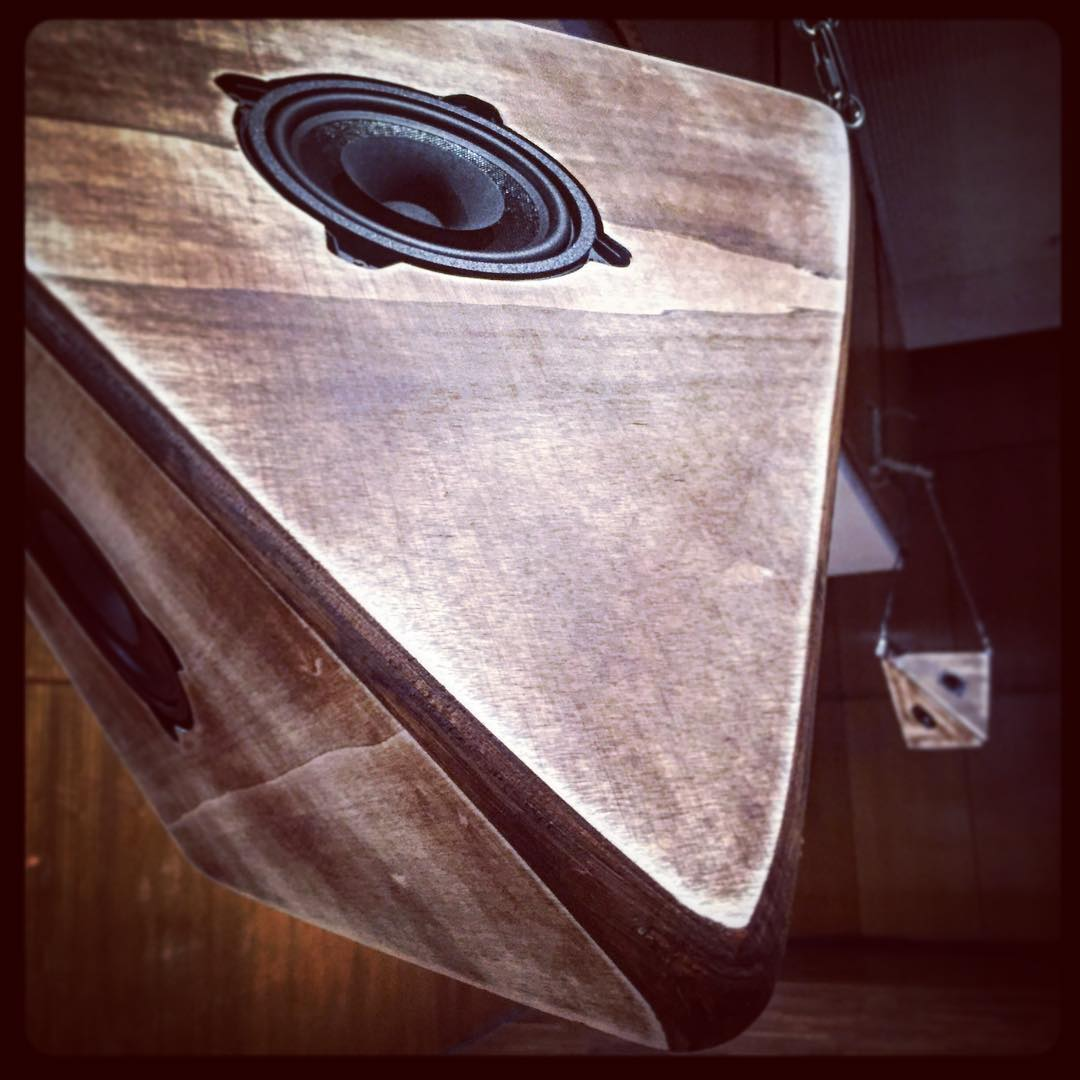
\includegraphics[width=.47\textwidth]{img/13556748_1807931906092757_1243460980_n.jpg}
\caption{S.T.ONE. Second prototype.}
\label{stone2}
\end{center}
\end{figure}

A traditional loudspeaker can be controlled only in the dynamic dimension of power and, by acting on it, a balance can be sought with acoustical instruments. Nevertheless, acoustical instruments have infinitely more complex behaviour, which implies time-relationships between the dynamics and the timbral character and, above all, the rhythm complexity of time-space factors of sound propagation till perception.

S.T.ONE (Spherical Tetrahedral ONE) is the result of a personal research aimed at solving this problem by allowing musical exposures in which the fusion between the two subjects, acoustic and electroacoustic, is total, multi-dimensional. The project was born from the need to be able to perform music by exploiting the sound space created by the electronic medium with perceptive acoustic characteristics similar to those of traditional instruments. With the S.T.ONE loudspeaker you can control the propagation of the sound reproduced in all directions of the space and allow you to integrate this control into the composition parameters in a dialectical relationship with the acoustic instrument.

\begin{figure}[htbp]
\begin{center}
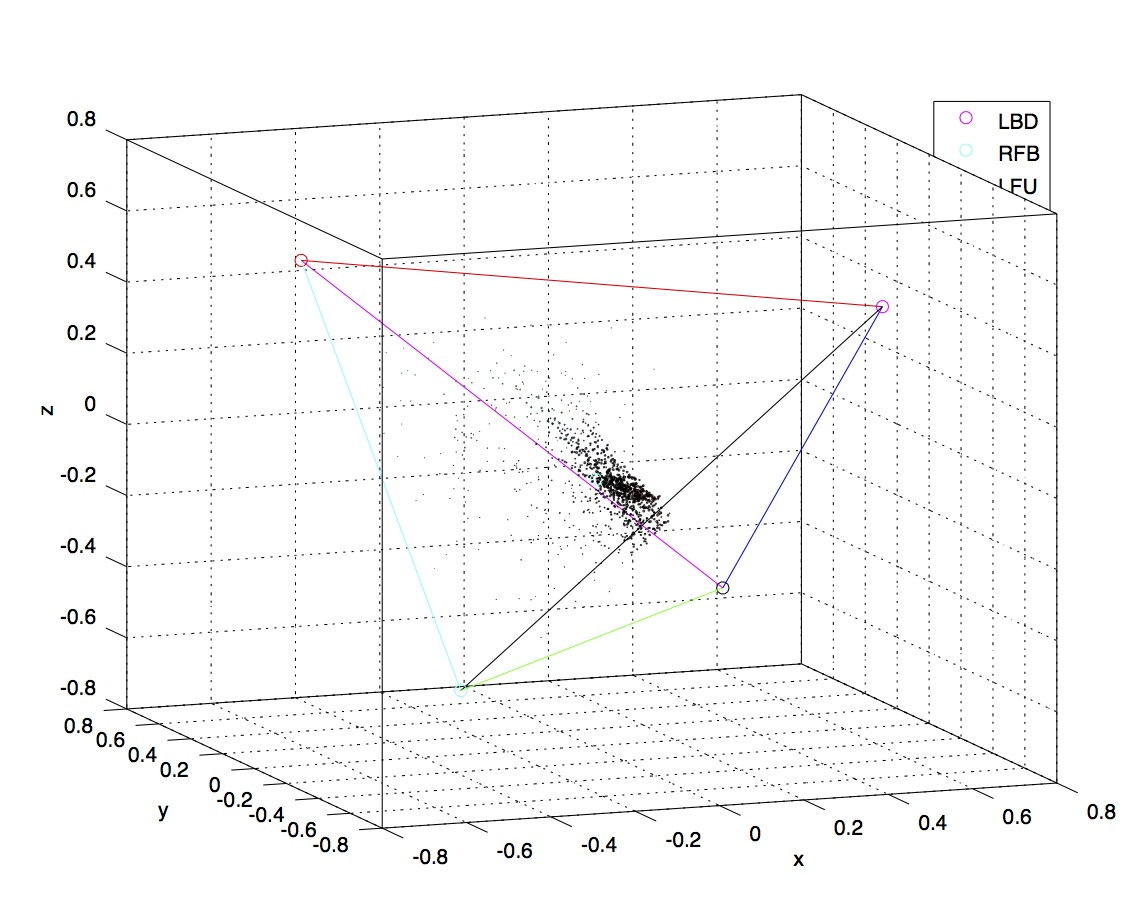
\includegraphics[width=.47\textwidth]{img/13230_1024_2.jpg}
\caption{A flute sound-shape visualization in four-dimensional space}
\label{shape}
\end{center}
\end{figure}

The second step of writing outline the concept of sound shape, which is the corpus of the entire research: the idea of sound micro-formal time-related with a multidimensional shape hardcoded by the relationship between the characteristics which produced it. 

In this slice of research will be sketched out the necessity to overcome traditional electroacoustic approach to sound diffusion and reproduction to observe the possibilities to reproduce sound shapes and time-variant micro-rhythm of sound. 

The third phase takes place on the two above expressed. In that article will be presented the TETRAREC, a spaced microphone technique able to capture sound shape of an acoustical system, I designed to imprint in audio recordings the sound shape of acoustical objects, even obviously musical instruments. 

I had only a few attempts to use the TETRAREC technique in studio circumstances and only one in real-time sound amplification. The RITMO facilities will be precious to develop and produce tons of recordings to be observed and analyzed. 

\emph{TETRAREC} is a spaced microphone technique which consists in surrounding the complex sound object (musician plus instrument) with four non-directional microphones, each at the vertices of an ideal tetrahedron.

The \emph{TETRAREC} technique took its inspiration from Michael Gerzon's \emph{A-Format} (four coincident microphones placed along the sides of a tetrahedron). The difference between the two techniques are the distance (coincident vs. spaced) and the purpose (3D reproduction of music/environment vs. 3D reproduction of acoustic objects)

The \emph{TETRAREC} technique was developed to achieve the following objectives:

\begin{compactitem}
\item Capture the \emph{sound-shape} of acoustic instruments
\item Preserve the body shadow on sound propagation
\item Preserve the movements performed by the musician
\item Collect data on \emph{sound-shapes} of different acoustic instruments
\item Collect data on \emph{sound-shapes} of similar acoustic instruments with different performers
\item Analyse data and prototype a graphic visualisation of 3D \emph{sound-shapes}
\item Capture sounds to be listened in a point of view, for virtual-reality environment
\end{compactitem}

%----------------------------------------------------------------------------------------
COMPLEXITY PERCEPTION

The sound shape stands out in the surrounding space and expands and moves within this space and it is modelled as a soft mass inside a container. Here the phenomena of reflection occur and the form crystallizes assuming characteristics in the function of space and, therefore, of time. The listener who takes part in this event sees acoustic listening heard in the space and feels the solid form coming from the instrumental body and at the same time, immediately afterwards, from the room in the form of reflections. A ritual, that of listening, which cannot do less than any of these details.

\clearpage
\section*{UNISOLO}
at the depth of every literature, the time

%----------------------------------------------------------------------------------------
\section{APPUNTI}
In addition, your research outline may also include:
Literature references (max 2,000 characters)
(The reference list must be sorted alphabetically by author.)
Word count

To count the number of characters in a text in MS Word, go to Review, and select Word Count. 9,000 characters with spaces is approximately three pages of text written in Times, 12-point type, with one and a half line spacing.

\bibliographystyle{IEEEbib}
%http://cim.lim.di.unimi.it
\bibliography{ttt.bib} % requires file lac-20.bib

\end{document}
